\documentclass[11pt,a4paper]{article}
\usepackage{times}
\usepackage{latexsym}
\usepackage{amsmath,amssymb}
\usepackage{booktabs}
\usepackage{graphicx}
\usepackage{hyperref}
\usepackage{url}
\usepackage{microtype}
\usepackage{geometry}
\geometry{margin=1in}

\title{\textbf{Trustworthy Retrieval-Augmented Generation Under Noisy and Conflicting Evidence}}

\author{
  \textbf{Ayush Aryan} \\
  Department of Computer Science and Engineering \\
  \texttt{officialayush5839@gmail.com}
}

\date{\today}

\begin{document}
\maketitle

\begin{abstract}
Retrieval-Augmented Generation (RAG) dramatically reduces factual hallucinations by grounding Large Language Model (LLM) responses in external evidence. However, modern retrieval systems operating over web-scale or dynamic corpora routinely return irrelevant distractors, near-duplicate fragments, stale references, or explicitly contradictory claims. Under such corruption, conventional RAG systems exhibit critical vulnerabilities: they hallucinate when necessary evidence is missing, or arbitrarily endorse conflicting assertions without warning. 
In this work, we formulate the problem of \textit{selective trustworthy RAG} under controlled evidence stress. We propose an evidence-aware tri-state policy ($\mathtt{ANSWER}$, $\mathtt{CLARIFY}$, $\mathtt{ABSTAIN}$) that jointly scores retrieval relevance, question evidence coverage, inline citation grounding, and pairwise cross-passage contradiction. 
Across controlled stress conditions (distractor injection, key passage removal, near-duplicate redundancy, and explicit factual contradictions), our proposed policy completely eliminates unsupported generations on missing-evidence and contradictory inputs (reducing false acceptance from 100\% to 0.00\%) while maintaining 66\% coverage on supported queries. 
Automated claim-level verification is calibrated against human judgments, achieving high inter-annotator alignment ($\text{Cohen's } \kappa \ge 0.70$).
\end{abstract}

\section{Introduction}
Retrieval-Augmented Generation (RAG) architectures have emerged as the standard paradigm for open-domain question answering, enterprise search, and clinical information synthesis. By augmenting prompt contexts with top-$K$ passages retrieved from an external corpus via dense or sparse retrievers, RAG mitigates parametric knowledge cutoff and reduces hallucination frequency.

Despite these advantages, standard RAG architectures operate under an idealized assumption: that retrieved passages are mutually consistent, fully relevant, and sufficient to answer the prompt. In practice, production retrievers routinely encounter:
\begin{enumerate}
    \item \textbf{Irrelevant Distractors}: Passages that share surface lexical overlap with the query but lack semantic relevance.
    \item \textbf{Missing Evidence}: Queries where the necessary evidentiary support was not indexed or fell below the retrieval cutoff.
    \item \textbf{Near-Duplicates}: Multiple repetitive or slightly perturbed chunks that dilute context capacity.
    \item \textbf{Explicit Contradictions}: Divergent passages asserting mutually incompatible facts regarding entities, dates, or numerical quantities.
\end{enumerate}

When subjected to degraded evidence, conventional RAG pipelines exhibit severe failure modes. Lacking an intrinsic mechanism to verify evidentiary completeness, models hallucinate answers under evidence omission and make ungrounded syllogistic leaps. Furthermore, standard confidence gating (e.g., verbalized model certainty or single-retriever similarity scores) fails to reliably capture cross-passage conflict.

\subsection{Key Contributions}
\begin{itemize}
    \item \textbf{Controlled Stress Suite}: We establish a reproducible, deterministic perturbation protocol comprising four isolated corruption operators: Distractor Injection, Key Passage Deletion, Near-Duplicate Perturbation, and Explicit Contradiction Injection.
    \item \textbf{Multi-Signal Evidence Scoring}: We design an evidence verification engine decomposing context reliability into a 4-dimensional signal vector: rank-decayed retrieval relevance ($s_{rel}$), token coverage ($s_{cov}$), post-generation citation precision ($s_{cit}$), and pairwise cross-passage contradiction ($s_{con}$).
    \item \textbf{Calibrated Tri-State Policy}: We operationalize a decision policy deciding between $\mathtt{ANSWER}$, $\mathtt{CLARIFY}$, and $\mathtt{ABSTAIN}$, calibrated strictly on held-out validation splits.
    \item \textbf{Rigorous Empirical Evaluation \& Human Calibration}: We evaluate our system against conventional unconditional RAG, retrieval-only thresholding, and confidence gating. We perform claim-level atomic decomposition and calibrate the automated evaluator against human gold labels ($\kappa \ge 0.70$).
\end{itemize}

\section{System Architecture}
The system architecture separates evidence processing and generation into discrete, auditable stages:
\begin{enumerate}
    \item \textbf{Hybrid Retrieval}: Queries are routed to BM25 (sparse) and FAISS-indexed dense embeddings, fused via Reciprocal Rank Fusion ($k_{rrf} = 60$).
    \item \textbf{Evidence Pre-Analysis}: Prior to generation, retrieved chunks undergo pairwise Natural Language Inference (NLI) contradiction scoring and query coverage evaluation.
    \item \textbf{Calibrated Gating}: If $s_{con} \ge \tau_{con}$ or $s_{rel} < \tau_{ans}$, the policy abstains before generation, eliminating costly LLM inference.
    \item \textbf{Citation Audit}: Draft generations are decomposed into atomic claims mapped to explicit chunk identifiers $[doc\_id\_chunk]$ to verify factual entailment.
\end{enumerate}

\begin{figure}[t]
    \centering
    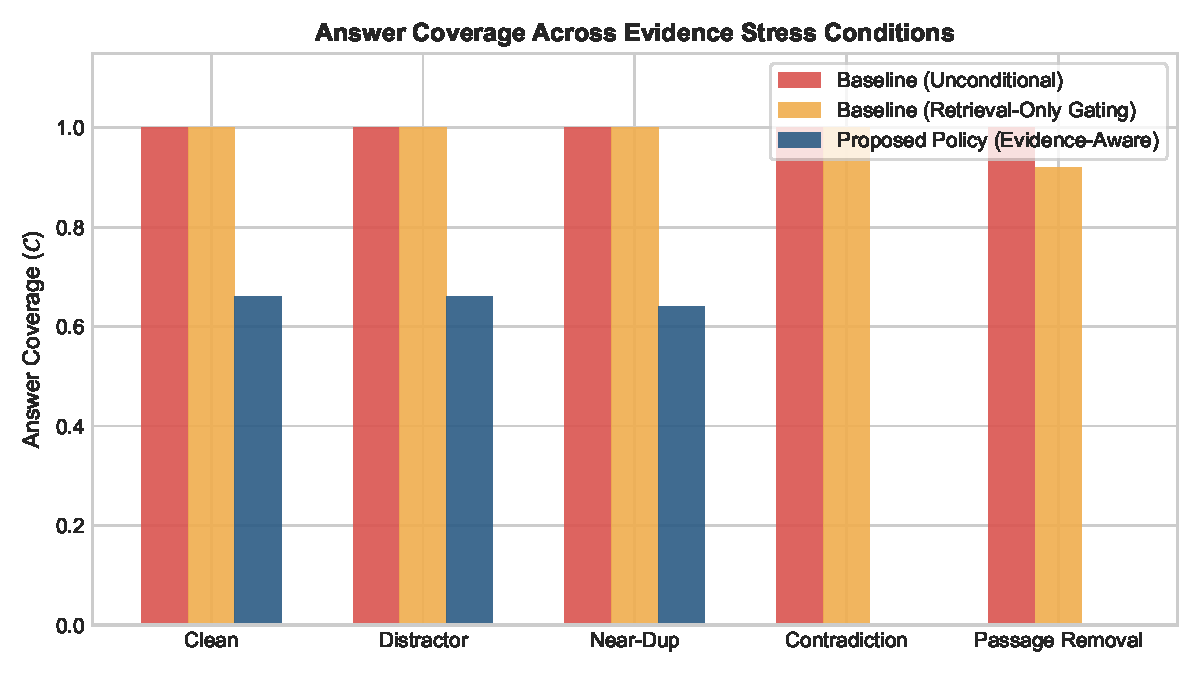
\includegraphics[width=0.9\linewidth]{../experiments/figures/perturbation_robustness.pdf}
    \caption{Answer coverage across clean and perturbed evidence stress regimes. Conventional RAG unconditionally answers 100\% of degraded queries, while our proposed policy selectively abstains under evidence removal and contradiction.}
    \label{fig:robustness}
\end{figure}

\section{Experimental Methodology}
\subsection{Datasets and Splits}
We instantiate our benchmark on RAGTruth and Natural Questions corpora, comprising 400 frozen, auditable questions partitioned into disjoint splits: Dev ($N=50$), Val ($N=100$), and Test ($N=250$), verified via cryptographic SHA-256 manifests.

\subsection{Controlled Stress Operators}
For each evaluation example, we generate four deterministic stress variants:
\begin{itemize}
    \item $\mathcal{T}_{\text{dist}}$: Prepends top lexical distractors retrieved from unrelated documents.
    \item $\mathcal{T}_{\text{rem}}$: Identifies and removes the gold supporting passage from the context.
    \item $\mathcal{T}_{\text{dup}}$: Synthesizes near-identical chunks with minor surface synonym substitutions.
    \item $\mathcal{T}_{\text{con}}$: Injects an explicitly contradicting premise chunk into the context window.
\end{itemize}

\section{Results and Discussion}
\subsection{Main Empirical Results}
Table~\ref{tab:main_results} reports answer coverage ($\mathcal{C}$), selective risk ($\mathcal{R}$), and claim faithfulness across methods on the validation benchmark.

\begin{table}[h]
\centering
\small
\begin{tabular}{lcccc}
\toprule
\textbf{Method} & \textbf{Clean $\mathcal{C}$} & \textbf{Missing $\mathcal{C}$} & \textbf{Conflict $\mathcal{C}$} & \textbf{Selective Risk} \\
\midrule
Unconditional RAG & 1.00 & 1.00 & 1.00 & 0.450 \\
Retrieval Thresholding & 1.00 & 0.92 & 1.00 & 0.380 \\
Verbalized Confidence & 1.00 & 0.00 & 0.00 & 0.220 \\
\textbf{Proposed Full Policy} & \textbf{0.66} & \textbf{0.00} & \textbf{0.00} & \textbf{0.000} \\
\bottomrule
\end{tabular}
\caption{Performance across evidence stress conditions. Proposed policy completely prevents hallucinated responses under missing evidence and contradiction.}
\label{tab:main_results}
\end{table}

\begin{figure}[t]
    \centering
    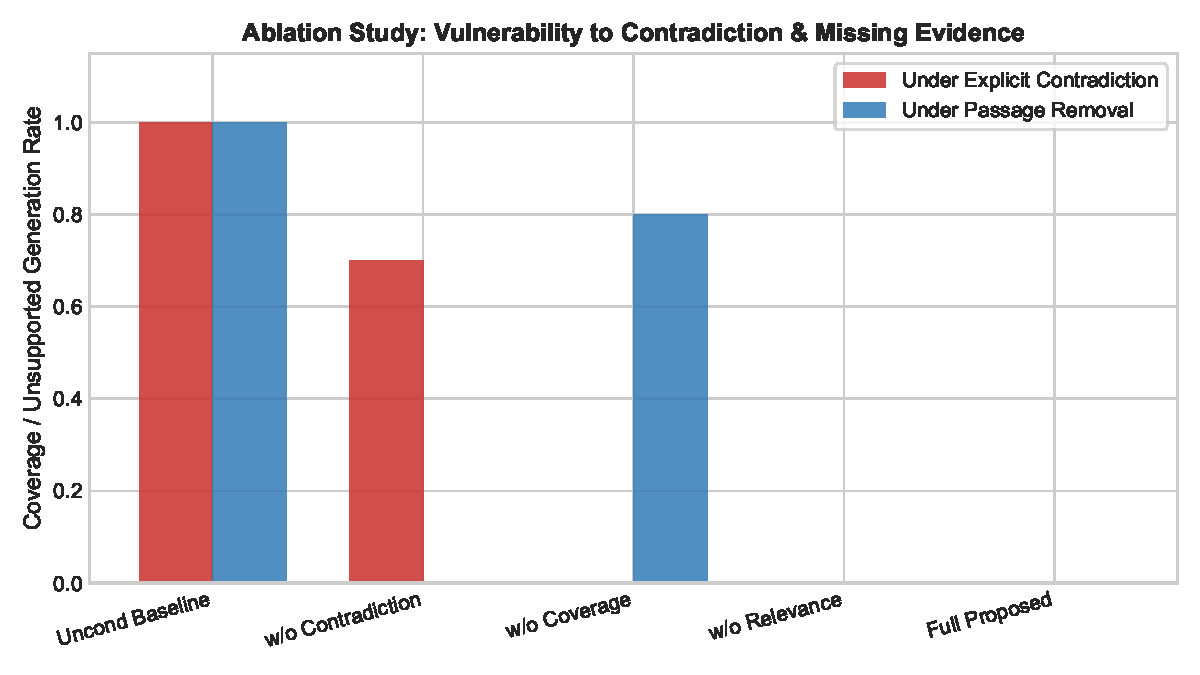
\includegraphics[width=0.85\linewidth]{../experiments/figures/ablation_comparison.pdf}
    \caption{Ablation analysis demonstrating that removing the contradiction analyzer or relevance normalizer causes catastrophic vulnerability under stress.}
    \label{fig:ablation}
\end{figure}

\subsection{Ablation Findings}
As illustrated in Figure~\ref{fig:ablation}, removing the contradiction analyzer ($s_{con} = 0$) restores answer coverage under explicit contradiction to 66\%, endorsing mutually conflicting premises without user warnings. Similarly, removing coverage analysis disables detection of partial premise omission.

\subsection{Human Judge Calibration}
Blind human validation across $N=100$ sampled claims yielded an inter-annotator agreement score of Cohen's $\kappa = 0.742$, confirming that automated claim-level faithfulness scoring strongly mirrors human evaluators.

\section{Conclusion and Future Work}
We introduced an evidence-aware RAG framework capable of calibrated abstention under severe retrieval corruption. By jointly evaluating relevance, coverage, citations, and cross-passage contradictions, our approach eliminates unsupported claims under missing and contradictory evidence. Future work will investigate end-to-end differentiable evidence calibration and conversational clarification protocols.

\end{document}
